\section{Point-Set Topology}

\begin{center}
    Notes from \textbf{Math 490: Introduction to Topology}

    Taken at University of Michigan, Fall 2025
\end{center}

\subsection{Metric Spaces}

\begin{framed}
\begin{defn}
    Let $X$ be a set. A \textbf{metric} is a function \[d:X\times X\to\mathbb{R}\] satisfying the following conditions for all $x,y,z\in X$:
    \begin{enumerate}
        \item[]\textbf{Positivity.} $d(x,y)\geq 0$ and $d(x,y)=0$ if and only if $x=y$
        \item[]\textbf{Symmetry.} $d(x,y) = d(y,x)$
        \item[]\textbf{Triangle Inequality.} $d(x,y)+d(y,z) \geq d(x,z)$
    \end{enumerate}
    A set $X$ with a metric $d$ is called a \textbf{metric space}, denoted $(X,d)$.
\end{defn}
\end{framed}

$d$ is sometimes called the \textit{distance} from $x$ to $y$. The most familiar metric, the \textbf{Euclidean metric}, mapping from $\mathbb{R}^n\times\mathbb{R}^n$, is given by \begin{equation*}
    d(\vec{x},\vec{y}) = \magnitude{\vec{x}-\vec{y}} = \sqrt{(x_1-y_1)^2+\dots+(x_n-y_n)^2}\hspace{1in}\text{(Euclidean Metric)}
\end{equation*} Note that the Euclidean metric is indeed a metric, and thus $(\mathbb{R}^n,d)$ is a metric space:
\begin{proof}
    Let $d:\mathbb{R}^n\times\mathbb{R}^n\to\mathbb{R}$ such that $d(\vec{x},\vec{y}) = \magnitude{\vec{x}-\vec{y}}$. Let $\vec{x},\vec{y},\vec{z}\in\mathbb{R}^n$.
    \vspace{-1em}
    \begin{enumerate}
        \item[] \textbf{Positivity}. Note that $d(\vec{x},\vec{y}) = \magnitude{\vec{x}-\vec{y}} = \sqrt{(x_1-y_1)^2+\dots+(x_n-y_n)^2}$. For any $a,b\in\mathbb{R}$, $(a-b)^2\geq 0$, so $\sqrt{(x_1-y_1)^2+\dots+(x_n-y_n)^2} \geq \sqrt{0} = 0$, so $d(\vec{x},\vec{y})\geq 0$.
        
        
        Suppose $\vec{x}=\vec{y}$. Then $x_1-y_1 = \dots = x_n-y_n=0$, so $d(\vec{x},\vec{y}) = \sqrt{(x_1-y_1)^2 + \dots + (x_n-y_n)^2} = \sqrt{0} = 0$. 
        
        Now suppose instead that $d(\vec{x},\vec{y})=0$. Then, $\sqrt{(x_1-y_1)^2+\dots+(x_n-y_n)^2} = 0$. Since $(a-b)^2$ is nonnegative for all $a,b\in\mathbb{R}$, then $(x_1-y_1)^2+\dots+(x_n-y_n)^2 = 0$ implies $x_1-y_1 = \dots = x_n-y_n = 0$. Thus, $\vec{x}-\vec{y} = 0$, or $\vec{x}=\vec{y}$.

        Thus, $d$ satisfies positivity.
        \item[] \textbf{Symmetry}. Note that $(a-b)^2=(b-a)^2$ for all $a,b\in\mathbb{R}$. Thus, $d(\vec{x},\vec{y}) = \sqrt{(x_1-y_1)^2+\dots+(x_n-y_n)^2} = \sqrt{(y_1-x_1)^2 + \dots + (y_n-x_n)^2} = d(\vec{y},\vec{x})$.
        \item[] \textbf{Triangle Inequality}. Note that: \begin{eqnarray*}
            d(\vec{x},\vec{z})^2 &=& (x_1-z_1)^2 + \dots + (x_n-z_n)^2\\
            &=& (x_1-y_1 + y_1 -z_1)^2 + \dots + (x_n - y_n + y_n -z_n)^2\\
            &=& (x_1-y_1)^2 + (y_1-z_1)^2 + 2(x_1-y_1)(y_1-z_1) + \dots + (x_n-y_n)^2 + (y_n-z_n)^2 + 2(x_n-y_n)(y_n-z_n)\\
            &=& (x_1-y_1)^2 + \dots + (x_n-y_n)^2 + 2\left[(x_1-y_1)(y_1-z_1) + \dots + (x_n-y_n)(y_n-z_n)\right]\\
            &\leq& d(\vec{x},\vec{y})^2 + d(\vec{y},\vec{z})^2 + 2d(\vec{x},\vec{y})d(\vec{y},\vec{z})\\
            &=& (d(\vec{x},\vec{y})+d(\vec{y},\vec{z}))^2
        \end{eqnarray*} Because square roots are increasing and squares are strictly nonnegative, by taking square roots we have $d(\vec{x},\vec{z})\leq d(\vec{x},\vec{y})+d(\vec{y},\vec{z})$.
    \end{enumerate}
\end{proof}

The following definitions define what it means for a subset of a metric space to be open or closed (or neither, or both). These definitions are particularly useful because they generalize the properties of open and closed intervals of Euclidean space to any metric space.
\begin{defn}
    \textbf{(Open Ball)}. Let $(X,d)$ be a metric space. Let $x_0\in X$. Let $r>0$. Then, the \textbf{open ball} of radius $r$ about $x_0$ is the subset of $X$ defined by \[B_r(x_0) = \{x\in X\mid d(x_0,x)<r\}\subseteq X\]
\end{defn}

\begin{defn}
    \textbf{(Interior Point and Open Sets in a Metric Space)}. Let $(X,d)$ be a metric space. Let $U\subseteq X$. A point $u\in U$ is called an \textbf{interior point} of $U$ if there exists some radius $r_u>0$ such that $B_r(u)\subseteq U$. The set $U\subseteq X$ is called \textbf{open} if every point $u\in U$ is an interior point of $U$.
\end{defn}

\begin{defn}
    \textbf{(Closed Sets in a Metric Space)}. A subset $U\subseteq X$ is \textbf{closed} if its complement $X\backslash U$ is open.
\end{defn}
Note that it is possible for a set to be both open and closed, or neither open nor closed. In other words, openness and closure are \textit{not} mutually exclusive.

\begin{defn}
    \textbf{(Accumulation and Isolation Points of a Set)}. Let $(X,d)$ be a metric space. Let $S\subseteq X$ be a set. A point $x\in X$ is an \textbf{accumulation point} of $S$ if for all $r>0$, the open ball $B_r(x)$ contains a point of $S$ distinct from $x$. An element $s\in S$ which is not an accumulation point of $S$ is called an \textbf{isolated point} of $S$ if there exists $r>0$ such that $B_r(s)$ contains no points of $S$ except for $s$.
\end{defn}

Note that, by definition, an isolation point of $S$ must be an element of $S$, but an accumulation point of $S$ need not be an element of $S$. For example, the interval $S=(0,1)\subseteq \mathbb{R}$ has accumulation points $[0,1]$, even thought $0,1\notin S$.

\begin{defn}
    \textbf{("The" Product Metric)}. Let $(X,d_X)$ and $(Y,d_Y)$ be metric spaces. Then, the Cartesian product $X\times Y$ may be endowed with a metric $d_{X\times Y}: (X\times Y)\times (X\times Y)\to \mathbb{R}$, most commonly defined by \[d_{X\times Y}((x_1,y_1),(x_2,y_2)) = \sqrt{d_X(x_1,x_2)^2+d_Y(y_1,y_2)^2}\]
\end{defn}

With these definitions, it is possible to discuss \textbf{continuity} on a metric space. Note that there are several equivalent definitions of continuity, but the most simple definition is essentially a generalization of the definition of continuity on the real number line.

\begin{shaded}
    \textbf{Continuity of functions}. Let $(X,d_X)$ and $(Y,d_Y)$ be metric spaces. Let $x,x'\in X$.
    
    \begin{defn}
        \textbf{($\varepsilon\delta$ Continuity)}. A function $f:X\to Y$ is called \textit{continuous at $x$} if, for all $\varepsilon>0$, there exists $\delta>0$ such that, if $d_X(x,x')<\delta$, then $d_Y(f(x),f(x'))<\varepsilon$. $f$ is called \textit{continuous} if it is continuous at every $x\in X$.
    
        A function which is continuous also satisfies the following equivalent definitions:\vspace{-1em}
        \begin{enumerate}
            \item $f$ is continuous if for all $\varepsilon>0$, there exists $\delta>0$ such that $f(B_\delta(x))\subseteq B_\varepsilon(f(x))$.
            \item $f$ is continuous if, given any open set $U\subseteq Y$, $f^{-1}(U)\subseteq X$ is open.
            \item $f$ is continuous if, given any open ball $B=B_r(y)\subseteq Y$, its preimage $f^{-1}(B)$ is an open subset of $X$.
        \end{enumerate}
    \end{defn}
\end{shaded}
Note that, considering the real numbers under the Euclidean metric, the $\varepsilon\delta$ definition of continuity reduces to the familiar definition of continuity. Using this analogy, alternative definition (1) becomes fairly obvious: if a point is within the $\delta$-ball, its image maps within the $\varepsilon$-ball. 

Alternative definition (2) is particularly useful, as it will generalize to spaces which do not have a notion of distance (i.e. generalized topological spaces). Because of its importance, a proof of alternative definition (2) is provided.
\begin{framed}
\newpage\begin{proof}
    Let $(X,d_X)$ and $(Y,d_Y)$ be metric spaces.
    
    Suppose $f$ is continuous. Let $U\subseteq Y$ be open. If $x\in f^{-1}(U)$, then $f(x)\in U$. Since $U$ is open, there exists $\varepsilon>0$ such that $B_\varepsilon(f(x))\subseteq U$. Since $f$ is continuous, for all $\varepsilon>0$ there exists $\delta>0$ such that $f(B_\delta(x))\subseteq B_\varepsilon(f(x))$. Thus, $f(B_\delta(x))\subseteq U$. Therefore, $B_\delta(x)\subseteq f^{-1}(U)$. Therefore, $x$ is an interior point of $f^{-1}(U)$, so $f^{-1}(U)$ is open.


    Suppose $f$ is a function such that, for any open set $U\subseteq Y$, $f^{-1}(U)\subseteq X$ is open. Let $x\in X$. Fix $\varepsilon>0$. Because the preimage of an open set is open, by assumption we have that $f^{-1}(B_\varepsilon(f(x)))$ is open because open balls are open. Since $x\in f^{-1}(B_\varepsilon(f(x)))$, $x$ is an interior point of $f^{-1}(B_\varepsilon(f(x)))$. Therefore, there exists $\delta>0$ such that $B_\delta(x)\subseteq f^{-1}(B_\varepsilon(f(x)))$. Therefore, $f(B_\delta(x))\subseteq B_\varepsilon(f(x))$.

    Therefore, the $\varepsilon\delta$ definition of continuity holds if and only if for all open sets $U\subseteq Y$, the preimage $f^{-1}(U)$ is open. Therefore, the two definitions are equivalent.
\end{proof}
\end{framed}

Similarly to continuity, a convergent sequence in a metric space can be defined by extending the familiar definition from analysis.
\begin{defn} \textbf{(Convergent Sequences)}. Let $(X,d)$ be a metric space. Let $(x_n)$ be a sequence indexed by the natural numbers. The sequence \textit{converges} to $x_\infty$, denoted $\lim_{n\to\infty} x_n = x_\infty$, if, for all $\varepsilon>0$, there exists $N>0$ such that, if $n>N$, then $d(x_n,x_\infty)<\varepsilon$.
\end{defn}
Note that, for the metric space $\mathbb{R}$ endowed with the Euclidean metric, the definition of convergence reduces to the definition from analysis. As with continuity, convergence may be equivalently defined with open sets.
\vspace{1em}
\begin{defn}
    \textbf{(Equivalent Definition of Convergence)}. Let $(X,d)$ be a metric space. A sequence $(x_n)$ is convergent if, for any open set $U\subseteq X$ which contains $x_\infty$, there exists some $N>0$ such that, if $n>N$, then $x_n\in U$.
\end{defn}
The definition of convergent sequences yields yet another (equivalent) definition for continuous functions:

\textbf{Sequence Definition of Continuity}. $f$ is continuous if, given any sequence $(x_n)$ of points in $X$ with limit $x_\infty\in X$, $\displaystyle\lim_{n\to\infty} f(x_n) = f(\displaystyle\lim_{n\to\infty} x_n)$.

The following is a useful criteria which can often be used to construct a convergent sequence in a metric space:

\textbf{Convergence Criteria for Sequences in Metric Spaces}. Suppose $(x_n)$ is a sequence of points in $X$ with the property that $x_n\in B_{\frac{1}{n}}(x)$. Then, $(x_n)$ converges to $x$. \begin{proof}
    Fix $\varepsilon>0$. Choose $N>\frac{1}{\varepsilon}$. Then, if $n>N$, $x_n\in B_\frac{1}{N}(x)$ and $d(x_n,x) < \frac{1}{N} < \varepsilon$. Therefore, $(x_n)$ converges to $x$.
\end{proof}

A similarly useful criteria characterizes \textit{closed} sets and is provided without proof. The criteria essentially provides a way to consider whether a set is closed without considering the complement set:

\textbf{Alternate Characterization of Closed Subsets}. A set $A\subseteq X$ is closed if any only if for any convergent sequence of points $(a_n)$ in $A$ converging to a point $a_\infty\in X$, the limit $a_\infty\in A$.

Note that many results which hold on $\mathbb{R}$ with the standard Euclidean metric do \textit{not} hold in a general metric space. For example, Cauchy sequences are \textit{not in general} equivalent to convergent sequences. In fact, $\mathbb{R}$ with the Euclidean metric is an example of a \textit{complete} metric space, a special type of metric space where Cauchy sequences are equivalent to convergent sequences.

\begin{shaded}
    \textbf{Complete Metric Spaces}. Let $(X,d)$ be a metric space. Let $(x_n)$ be a sequence in $X$.

    \begin{defn}
        \textbf{(Cauchy Sequence)}. $(x_n)$ is a Cauchy sequence if, for all $\varepsilon>0$, there exists $N>0$ such that, if $n,m>N$, then $d(x_n,x_m)<\varepsilon$.
    \end{defn}

    \begin{defn}
        \textbf{(Complete Metric Spaces)}. $(X,d)$ is a \textbf{complete} metric space if every Cauchy sequence in $X$ converges.
    \end{defn}

    \textbf{Fact}. If $(x_n)$ is a convergent sequence, $(x_n)$ is a Cauchy sequence.
\end{shaded}
A metric space fails to be complete if a sequence in $X$ is able to become arbitrarily close to a point not in $X$. In precisely this case, there exist Cauchy sequences which are not convergent. Specifically, in this case, there exist Cauchy sequences which limit to a point not contained in $X$, therefore failing to converge.

\begin{defn}
     Let $(X,d)$ be a metric space. Let $(x_n)$ be a sequence in $X$. Let $(n_i)$ be a strictly increasing sequence of natural numbers (note that $n_i\geq i$). The sequence $(x_{n_i})$ is called a \textbf{subsequence} of $(x_n)$.
\end{defn}
Familiarly, if $(x_n)$ converges to $x_\infty$, then any subsequence $x_{n_i}$ must also converge to $x_\infty$.

\begin{shaded}
    \textbf{Sequentially Compact Subspaces}. A metric space $(X,d)$ is called \textbf{sequentially compact} if every sequence in $X$ has a convergent subsequence. Similarly, a set $S\subseteq X$ is sequentially compact if every sequence of points in $S$ has a subsequence that converges to a point in $S$.

    A sequentially compact subspace $S\subseteq X$ has the following properties: \vspace{-1em}\begin{enumerate}
        \item \textbf{$S$ is closed}. That is, $X\backslash S$ is open.
        \item \textbf{$S$ is bounded}. That is, there exists $R>0$ such that, for every $x,y\in S$, $d(x,y)<R$.
    \end{enumerate}

    \begin{theorem*}
        \textbf{(Extreme Value Theorem for Metric Spaces)}. Let $C$ be a nonempty, sequentially compact subset of $X$. Let $f:X\to\mathbb{R}$ be a continuous function. Then, there exists a point $c\in C$ such that \[f(c)=\displaystyle\sup_{x\in C}f(x)\]
    \end{theorem*}

    \begin{theorem*}
        \textbf{Closed Subsets of Sequentially Compact Sets are Sequentially Compact}. Suppose that $(X,d)$ is a sequentially compact metric space, and $C\subseteq X$ is closed. Then, $C$ is sequentially compact.
    \end{theorem*}

    \begin{theorem*}
        \textbf{Sequentially Compact Implies Complete}. Suppose $(X,d)$ is a sequentially compact metric space. Then, it is complete.
    \end{theorem*}
\end{shaded}

On a subspace of $\mathbb{R}^n$, sequential compactness is equivalent to closure and boundedness (by the Heine-Borel theorem from analysis). Again, this result does \textit{not hold} for metric spaces in general.

\begin{theorem*}
    \textbf{Sequentially Compact Continuous Images are Sequentially Compact}. Suppose $f:X\to Y$ is a continuous function. If $C\subseteq X$ is sequentially compact, then $f(C)\subseteq Y$ is sequentially compact.
\end{theorem*} \begin{proof}
    Suppose $C$ is sequentially compact. Let $(c_n)$ be a sequence in $C$. Because $C$ is sequentially compact, there exists a subsequence $(c_{n_k})$ converging to $c_{n_\infty}\in C$. Since $f$ is continuous, $\displaystyle\lim_{n\to\infty}f(c_{n_k}) = f(c_{n_\infty})\in f(C)$. The choice of $(c_n)$ is arbitrary, so for any sequence $(f(c_n))$ in $f(C)$, there exists a subsequence $(f(c_{n_k}))$ in $f(C)$ converging in $f(C)$. Thus, $f(C)$ is sequentially compact.
\end{proof}

\newpage

\subsection{Topological Spaces}

\begin{framed}
\begin{defn}
    \textbf{Topological Space}. Let $X$ be a set. A \textit{topology} $\mathcal{T}$ on $X$ is a collection of subsets of $X$ that satisfies the following properties: \begin{enumerate}
        \item[] \textbf{The ambient space and empty set are open}. $\varnothing\in\mathcal{T}$ and $X\in\mathcal{T}$.
        \item[] \textbf{Arbitrary unions are open}. If $\{U_i\}_{i\in I}$ is any collection of elements of $\mathcal{T}$, then $\displaystyle\bigcup_{i\in I} U_i\in\mathcal{T}$
        \item[] \textbf{Finite intersections are open}. If $U_1,U_2\in \mathcal{T}$, then $U_1\cap U_2\in\mathcal{T}$.
    \end{enumerate} A set $X$ endowed with a topology $\mathcal{T}$ is called a \textbf{topological space} and is denoted $(X,\mathcal{T})$. A set $C\subseteq X$ is called \textbf{closed} if its complement $X\backslash C\in\mathcal{T}$.
\end{defn}
\end{framed}

Essentially, a topology specifies a space $X$ and the collection of subsets of $X$, i.e. those contained in $\mathcal{T}$, which are open. Note that $\mathcal{T}$ is a subset of the power set of $X$. Some examples of topologies on a set $X$ are listed: \begin{enumerate}
    \item[] The \textbf{indiscrete topology}, where the only open sets are $\varnothing$ and $X$. This topology is given by $\mathcal{T} = \{\varnothing,X\}$. This is the "coarsest" topology on $X$, containing the fewest allowable elements.
    \item[] The \textbf{discrete topology}, where \textit{every} subset of $X$ is open. This topology is given by the power set of $\mathcal{P}(X)$; i.e. $\mathcal{T} = \mathcal{P}(X) = \{U\mid U\subseteq X\}$. This is the "finest" topology on $X$, containing maximum elements (every subset of $X$, including singletons, is open).
    \item[] The \textbf{topology induced by a metric space}. Let $(X,d)$ be a metric space. Define $\mathcal{T}_d$ as the collection of all open sets in $X$ under the metric $d$. Then, $(X,\mathcal{T}_d)$ forms a topological space. A topology $\mathcal{T}$ on $X$ is called \textit{metrizable} if there exists a metric $d$ on $X$ such that $\mathcal{T}$ is the set $\mathcal{T}_d$ of open sets in the metric space $(X,d)$.
\end{enumerate}

\begin{framed}
\textbf{Example of Metrizability}. Let $X$ be a set. Consider the metrizability of the discrete and indiscrete topology:

The discrete topology \textit{is} metrizable. Let $d$ be the discrete metric, given by \[d(x,y) = \begin{cases}
    0,& x=y\\
    1,&x\neq y
\end{cases}\] Note that if $x\in X$, then $x\in B_\frac{1}{2}(x) = \{x\}$, so singletons are open. Because singletons are open, the union of singletons is open, so every set in $X$ is open with the discrete metric. Thus, $(X,d)$ induces the discrete topology.

The indiscrete topology is \textit{not} metrizable if $X$ contains at least two distinct elements. Let $d$ be any metric on $X$. If $x_1,x_2\in X$ are distinct, then for $r=d(x_1,x_2)$, $x_2\notin B_r(x_1)$ and $x_1\in B_r(x_1)$. Therefore, $B_r(x_1)\neq \varnothing$ and $B_r(x_1)\neq X$, so $d$ does not induce the indiscrete topology. The choice of metric is arbitrary, so the indiscrete topology is not metrizable.
\end{framed}

Note that the following properties hold in general topological spaces:
\vspace{-1em}
\begin{enumerate}
\item $X$ and $\varnothing$ are closed. \begin{proof}
        Note that $X\backslash X = \varnothing$ which is open. Therefore, $X$ is closed. Similarly, $X\backslash \varnothing = X$ which is open. 
        
        Therefore, $\varnothing$ is closed.
    \end{proof}
    \item If $B$ and $C$ are closed subsets of $X$, then $B\cup C$ is closed. \begin{proof}
        Note that $X\backslash (B\cup C) =  (X\backslash B) \cap (X\backslash C)$ which is a finite intersection of open sets and is therefore open. 
        
        Therefore, $B\cup C$ is closed.
    \end{proof}
    \item For a collection $\{C_i\}_{i\in I}$ of closed subsets of $X$, the arbitrary intersection $\displaystyle\bigcap_{i\in I} C_i$ is closed. \begin{proof}
        Note that $X\backslash \displaystyle\bigcap_{i\in I} C_i = \displaystyle\bigcup_{i\in I} (X\backslash C_i)$ by DeMorgan's laws, which is open. Therefore, $\displaystyle\bigcap_{i\in I} C_i$ is closed.
    \end{proof}
\end{enumerate}

\begin{shaded}
    \textbf{Subspace Topology}. Let $(X,\mathcal{T}_X)$ be a topological space. Let $S\subseteq X$. Then, $S$ inherits the structure of a topological space called the \textit{subspace topology}, $\mathcal{T}_S$, defined by: \[\mathcal{T}_S = \{U\cap S\mid U\in\mathcal{T}_X\}\]
\end{shaded}

It is often convenient to work with some collection of sets which \textit{generates} a topology, rather than with a topology itself. Such a generating set is called a \textit{basis} for a topology.

\begin{framed}
\begin{defn}
    \textbf{(Basis of a topology)}. Let $(X,\mathcal{T})$ be a topological space. A collection $\mathcal{B}$ of subsets of $X$ is called a \textbf{basis} for the topology $\mathcal{T}$ if:\vspace{-1em}\begin{enumerate}
        \item[-] $\mathcal{B}\subseteq \mathcal{T}$, so every basis element in open
        \item[-] Every element of $\mathcal{T}$ can be expressed as a union of elements of $\mathcal{B}$.
    \end{enumerate} The basis $\mathcal{B}$ "generates" the topology $\mathcal{T}$.
\end{defn}
\end{framed}
Note that the term "basis" is analogous to a "spanning set", as a basis for a topology has no requirement of minimality. In fact, the basis $\mathcal{B}=\mathcal{T}$ is a (trivial) example of a basis, and many topologies do not have a finite basis (and therefore a minimal basis does not necessarily exist). For example, a basis for the Euclidean topology on the real numbers contains infinitely many open intervals.

The following set of definitions generalize several concepts from metric spaces; for this reason, these definitions align with intuition on certain familiar metric spaces as Euclidean space, but in fact generalize concepts without a notion of distance (i.e. to non-metrizable topological spaces).

\begin{framed}
    Let $(X,\mathcal{T})$ be a topological space, and $A\subseteq X$.
    \begin{defn}
        \textbf{(Interior of a Set)}. The interior of $A$, denoted $\text{Int}(A)$, is defined as the set \[\text{Int}(A) = \{a\in A\mid a\text{ is an interior point of }A\}\] $\text{Int}(A)$ is an open set, and is essentially the "largest" open subset of $A$.
    \end{defn}

    \begin{defn}
        \textbf{(Closure of a Set)}. The closure of $A$, denoted $\overline{A}$, is defined as the set \[\overline{A} = \{x\in X\mid \text{every open neighborhood }U\text{ of }x\text{ contains a point of }A\}\] The closure $\overline{A}$ is a closed set, and is essentially the "smallest" closed set containing $A$.
    \end{defn}

    \begin{defn}
        \textbf{(Accumulation Points of a Set)}. The accumulation points of $A$, contained in the set denoted $A'$, are defined by \[A' = \{x\in X \mid \text{every open neighborhood }U\text{ of }x\text{ contains a point of } A\text{ distinct from }x\}\] 
    \end{defn}

    \begin{defn}
        \textbf{(Boundary of a Set)}. The boundary of $A$, denoted $\partial A$, is defined as the set \[\partial A = \{x\in X\mid \text{every open neighborhood }U\text{ of }x\text{ contains a point in }A\text{ and a point in }X\backslash A\}\] Note that $\partial A = \partial (X\backslash A)$, i.e. $\partial A$ is a "shared" boundary between $A$ and the ambient space.
    \end{defn}

    Note that every point of $X$ is contained in precisely one of: $\text{Int}(A)$, $\text{Int}(X\backslash A)$, or $\partial A = \partial (X\backslash A)$.
\end{framed}

By considering the equivalent open-set definition of continuity, the notion of continuous functions can immediately be generalized in a topological space. 
\begin{shaded}
    Let $(X,\mathcal{T}_X)$ and $(Y,\mathcal{T}_Y)$ be topological spaces. Let $f:X\to Y$. $f$ is called \textit{continuous} if, for every set $U\subseteq Y$ open in $Y$, $f^{-1}(U)\subseteq X$ is open in $X$.

    It can be shown that, equivalently, $f$ is continuous if for every closed set $C\subseteq Y$, $f^{-1}(C)\subseteq X$ is closed. 
\end{shaded}
\vspace{-1em}
By considering the open-set definition of sequential convergence, this notion is also immediately generalized.
\begin{shaded}
    Let $(X,\mathcal{T}_X)$ be a topological space. A sequence $(x_n)$ converges to $x_\infty$ if, for any open neighorhood $U\subseteq X$ of $x_\infty$, there exists some $N>0$ such that, if $n>N$ then $x_n\in U$.

    Note that, in a general topological space, \textit{limits are not necessarily unique.} That is, a sequence may converge to more than one limit.

    \textbf{Example (Sierpinski Topology)}. Consider the set $\mathbb{S}=\{0,1\}$ endowed with the topology $\mathcal{T}_\mathbb{S} = \{\varnothing, \{0\}, \{0,1\}\}$. Consider the following sequences: \[\{a_n\} = \{0,\ 0,\ 0,\ 0,\ \dots\},\hspace{0.25in}\{b_n\} = \{1,\ 1,\ 1,\ 1,\ \dots\},\hspace{0.25in} \{c_n\}= \{1,\ 0,\ 1,\ 0,\ \dots\}\] Note that the open neighborhoods of $0$ are $\{0\}$ and $\{0,1\}$. Then, we see that $(a_n)$ converges to $0$ because $a_n\in \{0\}$ and $a_n\in \{0,1\}$, so $(a_n)$ is contained in every open neighborhood of $0$ for all $n$. Similarly, the only open neighborhood of $1$ is $\{0,1\}$, and $a_n\in \{0,1\}$ for all $n$, so $(a_n)$ converges to $1$ as well.

    By similar logic, we can see that $(b_n)$ converges to $1$, and we also have that $(c_n)$ converges to $1$, which follows from the fact that the only open neighborhood containing $1$ is $\{0,1\}$, which is the whole space.
\end{shaded}

\begin{framed}
\textit{The Product Topology.} Let $(X,\mathcal{T}_X)$ and $(Y,\mathcal{T}_Y)$ be topological spaces. Then, the \textit{product topology} on $X\times Y$, denoted $\mathcal{T}_{X\times Y}$, is generated by the basis \[\mathcal{B} = \{U\times V\mid U\subseteq X\text{ is open, and }V\subseteq Y\text{ is open}\}\] Some special features of the product topology will be discussed.

\textit{Property 1.} Suppose $(X, d_X)$ and $(Y,d_Y)$ are metric spaces. Then, the product metric $d_{X\times Y}$ induces the product topology on $X\times Y$. That is to say, the product metric has the same structure as the product topology. For this reason, the following properties also apply to the product metric, but are shown in more generality here.

\textit{Property 2.} The projection maps $\pi_X:X\times Y\to X$, which maps $(x,y)\mapsto x$, and $\pi_Y:X\times Y\to Y$, which maps $(x,y)\mapsto y$, are continuous. \begin{proof}
    Without loss of generality, we show that $\pi_X$ is continuous. Let $U\subseteq X$ be an open subset of $X$. Then, $\pi^{-1}_X(U) = U\times Y$. Note that $U\subseteq X$ is open in $X$ and $Y\subseteq Y$ is open in $Y$, so $U\times Y\in\mathcal{B}$. Basis elements are open, so $U\times Y=\pi_X^{-1}(U)$ is open in the product topology on $X\times Y$. Our choice of $U$ is arbitrary, so $\pi_X$ is continuous.
\end{proof} The projection maps are often useful when something is known about $X$ or $Y$, but not their product; because they are continuous, the project maps allow one to work with subsets of either $X$ or $Y$ while preserving the structure of the topology.

\textit{Property 3.} A function $f:X\to Y_1\times Y_2$, given by $f(x) = (f_1(x), f_2(x))$ is continuous if and only if $f_1(x)$ and $f_2(x)$ are continuous. \begin{proof}
    Suppose $f$ is continuous. Then $\pi_{Y_1}(f)$ and $\pi_{Y_2}(f)$ are continuous, because the composition of continuous functions is continuous. Note that $\pi_{Y_1}(f) = f_1$ and $\pi_{Y_2}(f)=f_2$, so both $f_1$ and $f_2$ are continuous.

    Suppose $f_1$ and $f_2$ are continuous. Let $W\subseteq Y_1\times Y_2$ be any open subset. Note that $W$ can be expressed as a union of basis elements, so $W=\displaystyle\bigcup_{i\in I} (U_i\times V_i)$ for some index $I$, where each $U_i\subseteq Y_1$ is open and each $V_i\subseteq Y_2$ is open. Then, \[f^{-1}(W) = f^{-1}\left(\displaystyle\bigcup_{i\in I} (U_i\times V_i)\right) = \displaystyle\bigcup_{i\in I} f^{-1}(U_i\times V_i)\] Note that this is an arbitrary union of basis elements, so it suffices to show that $f^{-1}(U_i\times V_i)$ is open for an arbitrary basis element. Note that, if $x\in f^{-1}(U_i\times V_i)$, then $x\in f_1^{-1}(U_i)$ and $x\in f_2^{-1}(V_i)$. Then, $x\in f_1^{-1}(U_i) \cap f_2^{-1}(V_i)$. Note that $f_1^{-1}(U_i)$ is open and $f_2^{-1}(V_i)$ is open, so their finite intersection is open. Therefore, $f^{-1}(W)$ is open, so $f$ is continuous.

    Therefore, $f$ is continuous if and only if $f_1$ and $f_2$ are continuous.
\end{proof}
\end{framed}
\vspace{-2em}
\subsection{Structured Topological Spaces}

When the discussion of topological spaces is restricted to the less general case of topologies which have some additional structure, several useful results can be shown. 

\begin{framed}
    \textbf{Separation Axioms}. Let $(X,\mathcal{T}_X)$ be a topological space. Let $x,y\in X$ be any distinct points.
    \begin{enumerate}
        \item[] \textbf{$T_1$ Space}. $X$ is called $T_1$ if there exists an open neighborhood $U_x$ of $x$ that does not contain $y$, and an open neighborhood $U_y$ of $y$ that does not contain $x$.
        \item[] \textbf{$T_2$ Space}. $X$ is called $T_2$ if there exist disjoint open neighborhoods $U_x$ of $x$ and $U_y$ of $y$. This is called the \textbf{Hausdorff property}, and $T_2$ spaces are equivalently called Hausdorff spaces.
        \item[] \textbf{$T_3$ Space}. $X$ is called $T_3$ if it is a \textit{regular} $T_0$ space. $X$ is called \textit{regular} if, for every closed subset $C$ not containing $x$, there exist disjoint open subsets $U_x$ and $U_C$ containing $x$ and $C$, respectively.
        \item[] \textbf{$T_4$ Space}. $X$ is called $T_4$ if it is a normal $T_2$ space. $X$ is called \textit{normal} if, for any pair of disjoint closed subsets $C$ and $D$, there exist disjoint open sets $U_C$ and $U_D$ containing $C$ and $D$, respectively.
    \end{enumerate}
    There are more separation axioms, but these ones are sufficient for many results. In particular, $T_1$ and $T_2$ spaces have several nice properties which facilitate useful results. The separation axioms give strictly stronger conditions on disjoint open neighborhoods around distinct points. As a consequence, it can be shown that $T_4\implies T_3\implies T_2\implies T_1$, and so on for other separation axioms. The visual meaning of the separation axioms is shown below, where dotted balls represent open sets and solid boxes represent closed sets:
    \begin{center}
    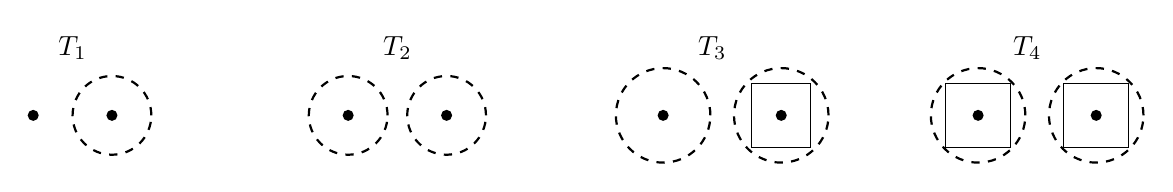
\begin{tikzpicture}[scale=1]

% ---------- T1 ----------
\node at (1,0.85) {$T_1$};

\draw[dashed, thick] (1.5,0) circle (0.5);
\fill (0.5,0) circle (2pt);
\fill (1.5,0) circle (2pt);

\node at (5.125,0.85) {$T_2$};

\draw[dashed, thick] (4.5, 0) circle (0.5);
\draw[dashed, thick] (5.75, 0) circle (0.5);
\fill (4.5, 0) circle (2pt);
\fill (5.75, 0) circle (2pt);

\node at (9.125,0.85) {$T_3$};

\draw[dashed, thick] (10, 0) circle (0.6);
\draw[dashed, thick] (8.5, 0) circle (0.6);
\fill (8.5, 0) circle (2pt);
\fill (10, 0) circle (2pt);
\draw (9.625, -0.41) rectangle (10.375, 0.41);

\node at (13.125,0.85) {$T_4$};

\draw[dashed, thick] (14, 0) circle (0.6);
\fill (12.5, 0) circle (2pt);
\fill (14, 0) circle (2pt);
\draw (13.59, -0.41) rectangle (14.41, 0.41);
\draw (12.09, -0.41) rectangle (12.91, 0.41);
\draw[dashed, thick] (12.5, 0) circle (0.6);

\end{tikzpicture}
\end{center}
\vspace{-1em}
A topology having the $T_1$ separation axiom is equivalent to the statement that "points are closed," i.e. every singleton is a closed set. \vspace{-1em}\begin{proof}
    Suppose $(X,\mathcal{T}_X)$ is $T_1$. Consider the singleton $\{x\}$. We wish to show that $X\backslash\{x\}$ is open, meaning any point $y\in X\backslash \{x\}$ is an interior point. Because $X$ is $T_1$, there exists an open neighborhood $U_y$ of $y$ which does not contain $x$. Then, $U_y\subseteq X\backslash \{x\}$ is an open neighborhood of $y$ contained in $X\backslash \{x\}$ and therefore $y$ is an interior point. Then, $X\backslash \{x\}$ is open, so $\{x\}$ is closed.

    Suppose $(X,\mathcal{T}_X)$ has the property that every singleton $\{x\}$ is closed. Then, $X\backslash \{x\}$ is open. Then, for every $y\in X$ distinct from $x$, $y$ is an interior point of $X\backslash \{x\}$. Then, there exists some open neighborhood $U_y$ of $y$ contained in $X\backslash \{x\}$. Then, $x\notin U_y$. Then, $X$ is $T_1$.

    Therefore, $X$ is $T_1$ if and only if points (i.e. singleton sets) are closed.
\end{proof}

Another important result is that metric spaces are $T_2$ topological spaces.\vspace{-1em} \begin{proof}
    Suppose $(X,d)$ is a metric space. Let $x,y\in X$ be distinct points. Let $r=d(x,y)/2$. We now show that $B_r(x)$ and $B_r(y)$ are disjoint open neighborhoods of $x$ and $y$ respectively.

    Suppose for sake of contradiction that $B_r(x)$ and $B_r(y)$ are not disjoint, so there exists some $z\in B_r(x)\cap B_r(y)$. Then, $d(z,x)< r$ and $d(z,y)<r$. By the triangle inequality, $d(x,z) + d(y,z) \geq d(x,y)$. But then, \[r+r > d(x,z)+ d(y,z) \geq d(x,y) = 2r\] Then, we have that $2r>2r$, which is not true. Therefore, no such $z$ can exist. Therefore, $B_r(x)\cap B_r(y)$ are disjoint. Clearly $B_r(x)$ is an open neighborhood of $x$, and clearly $B_r(y)$ is an open neighborhood of $y$, so there exist disjoint open neighborhoods of $x$ and $y$, specifically $B_r(x)$ and $B_r(y)$. Therefore, $(X,d)$ is $T_2$.
\end{proof}

To summarize, this results in the following theorems:

\textbf{Theorem}. Metric spaces are Hausdorff. Notably, if a topological space is not Hausdorff, it is not metrizable.

\textbf{Theorem}. A topological space is $T_1$ if and only if points are closed.

Note that, because $T_2\implies T_1$, points are closed in $T_2$ spaces as well.
\end{framed}

Hausdorff spaces tend to generalize many properties of metric spaces; in particular, Hausdorff spaces generalize the notion of "disjoint open balls" without the notion of distance. One such "nice" property is that sequences in Hausdorff spaces have unique limits.

\textbf{Theorem}. If $X$ is Hausdorff and $(x_n)$ is a convergent sequence, then its limit is unique.\vspace{-1em}
\begin{proof}
    Let $X$ be a Hausdorff space. Suppose $(x_n)$ converges to $a$ and $(x_n)$ converges to $b$. We seek to show that $a=b$.
    Assume for sake of contradiction that $a\neq b$. Since $X$ is Hausdorff, there exist disjoint open neighborhoods $U_a$ of $a$ and $U_b$ of $b$. Since $(x_n)$ converges to $a$, there exists $N_a>0$ such that if $n>N_a$, then $x_n\in U_a$. Similarly, there exists $N_b>0$ such that if $n>N_b$, then $x_n\in U_b$. Let $N=\max(N_a,N_b)$. Then, if $n>N$, we have that $x_n\in U_a$ and $x_n\in U_b$. However, we have that $U_a$ and $U_b$ are disjoint, which is a contradiction. Then, it must be the case that $a=b$, so limits are unique.
\end{proof}

\begin{shaded}
    \textbf{Connected and Path-Connected Subspaces}. Let $(X,\mathcal{T})$ be a topological space. We say that $X$ is \textbf{disconnected} if there exist disjoint, nonempty, open subsets $A$ and $B$ such that $X=A\cup B$. The sets $A$ and $B$ are a \textit{separation} of $X$. If no such separation exists, $X$ is called \textit{connected}. A \textit{connected component} of $X$ is the maximal connected subset of $X$ (and a disconnected set will have more than one connecting component).

    Two important results are given without proof:
    \vspace{-1em}
    \begin{enumerate}
        \item[-] $X$ is disconnected if and only if there exists a nontrivial subset $A$ which is both open and closed (i.e. there exists clopen $A$ where $A\neq\varnothing$ and $A\neq X$).
        \item[-] \textbf{Generalized Intermediate Value Theorem}. Let $X$ be connected and $f:X\to(\mathbb{R},\text{Euclidean})$ be continuous. If $x,y\in X$ and $f(x)<c<f(y)$, then there exists some $z\in X$ such that $f(z)=c$.
    \end{enumerate}
    \vspace{-1em}
    Let $X$ be a topological space, with $x,y\in X$. A \textit{path} from $x$ to $y$ is any continuous function $\gamma:([0,1],\text{Euclidean})\to (X,\mathcal{T})$ such that $\gamma(0)=x$ and $\gamma(1)=y$. The space $(X,\mathcal{T})$ is \textbf{path-connected} if given any $x$ and $y$, there exists a path from $x$ to $y$. 
    
    Three important results of path-connectedness are given without proof:
    \vspace{-1em}
    \begin{enumerate}
        \item[-] If $X$ is path-connected, then $X$ is connected. Note that the opposite is not true, i.e. there exists connected spaces which are \textit{not} path connected.
        \item[-] Suppose $f:X\to Y$ is a continuous map between topological spaces. If $X$ is path-connected, then $f(X)$ is path-connected.
        \item[-] The product $X\times Y$ with the product topology is connected if and only if both $X$ and $Y$ are connected.
    \end{enumerate}
\end{shaded}

\textbf{Definition (Open Cover)}. Let $(X,\mathcal{T})$ be a topological space. A collection $\{U_i\}_{i\in I}$ such that $\bigcup_{i\in I} U_i = X$ is called an \textit{open cover} of $X$. A sub-collection $\{U_i\}_{i\in I'}$, with $I'\subseteq I$, is called an \textit{open subcover} of $X$ if $\{U_i\}_{i\in I'}$ is also a cover of $X$.

Note that one can also talk about an open cover of some subset $A\subseteq X$. There are two equivalent ways to describe covers of $A$: either $A=\bigcup_{i\in I} U_i$ where each $U_i$ is open in the subspace topology $\mathcal{T}_A$, or $A\subseteq \bigcup_{i\in I} U_i$ where each $U_i$ is open in $X$. Note that every set has at least one cover, with the entire space $X$ being a trivial example.

\begin{framed}
    \textbf{Compactness}. A topological space $(X,\mathcal{T})$ is \textbf{compact} if \textbf{every} open cover of $X$ has a finite subcover.

    Several important results for compact spaces are outlined:

    \textbf{Theorem}. Closed subsets of compact spaces are compact. \vspace{-1em}\begin{proof}
        Let $(X,\mathcal{T})$ be a compact topological space. Suppose $A\subseteq X$ is closed. Let $\{U_i\}_{i\in I}$ be any open cover of $A$. We wish to show that there exists a finite subcover of $A$. $A$ is closed, so $X\backslash A$ is open. Since $\{U_i\}_{i\in I}$ is an open cover of $A$, we have that $(X\backslash A) \cup \left(\displaystyle\bigcup_{i\in I} U_i\right) = X$. Since this collection covers $X$, there exists a finite collection $(X\backslash A)\cup\left(\displaystyle\bigcup_{i\in I'} U_i\right)$ of sets which also covers $X$, where $I'\subseteq I$ is finite. Then, it must be the case that $A\subseteq \displaystyle\bigcup_{i\in I'}U_i$. Then, there exists some finite collection $\{U_i\}_{i\in I'}$ which is a finite subcover of $A$. Then, $A$ is compact.
    \end{proof}

    \textbf{Theorem}. A subset of a Hausdorff topological space is closed if and only if it is compact.

    \vspace{-1em}\begin{proof}
        Let $(X,\mathcal{T})$ be a Hausdorff topological space. We have already shown that, if $X$ is compact, then closed subsets are compact. We must only show that, if subsets are compact, then they are closed.

        Let $A\subseteq X$ be a compact subset of $X$. We seek to show that $A$ is closed, meaning $X\backslash A$ is open. Fix $x\in X\backslash A$. Because $X$ is Hausdorff, for every $a\in A$, there exist disjoint open neighborhoods $U_a$ of $a$ and $V_a$ of $x$. Note that $\{U_a\}_{a\in A}$ is an open cover of $A$, because every point of $A$ is included in some $U_a$. Because $A$ is compact, there exists some finite collection of points $a_1,\dots,a_n$ where $\{U_{a_i}\}_{i\leq n}$ is a finite subcover of $A$. Define $V=\displaystyle\bigcap_{i=1}^n V_{a_i}$. Note that $x\in V_{a_i}$ for each (finitely many) $i$, so $V$ is an open neighborhood of $x$ contained in $X\backslash A$. Then, $x$ is an interior point of $X\backslash A$. Our choice of $x$ is arbitrary, so $X\backslash A$ is open. Therefore, $A$ is closed.

        Therefore, we have that a subset of a compact Hausdorff space is compact if and only if it is closed.
    \end{proof}

    \textbf{Theorem}. Suppose $f:X\to Y$ is a continuous map between topological spaces. If $X$ is compact, then $f(X)\subseteq Y$ is compact. \vspace{-1em}\begin{proof}
        Let $X$ be compact, and let $f:X\to Y$ be a continuous function. Suppose $\{U_i\}_{i\in I}$ is an open cover of $f(X)$. Then, $f(X)\subseteq \displaystyle\bigcup_{i\in I} U_i$. Then, $X = f^{-1}(f(X))\subseteq f^{-1}\left(\displaystyle\bigcup_{i\in I} U_i\right) = \displaystyle\bigcup_{i\in I} f^{-1}(U_i)$ Note that this follows because $X\subseteq f^{-1}(f(X))$ is a property of preimages, and $f$ is defined on $X$ so $f^{-1}(U_i)\subseteq X$ for each $i\in I$. Because $f$ is continuous, $f^{-1}(U_i)$ is open for each $i\in I$, and we have that $\displaystyle\bigcup_{i\in I}f^{-1}(U_i) = X$, so $\{f^{-1}(U_i)\}_{i\in I}$ is an open cover of $X$. Because $X$ is compact, there exists some finite $I'\subseteq I$ where $\{f^{-1}(U_i)\}_{i\in I'}$ is a finite subcover of $X$. Because $X\subseteq\displaystyle\bigcup_{i\in I'} f^{-1}(U_i)$, we have that $f(X)\subseteq \displaystyle\bigcup_{i\in I'} U_i$. Therefore, $\{U_i\}_{i\in I'}$ is a finite subcover of $f(X)$. Therefore, $f(X)$ is compact.
    \end{proof}

    A final result is presented without proof.

    \textbf{Generalized Extreme Value Theorem}. Let $X$ be a nonempty compact topological space, and $f:X\to(\mathbb{R},\text{Euclidean})$ be continuous. Then, $\sup(f(X))$ is finite, and there exists some $z\in X$ such that $f(z)=\sup(f(X))$.
\end{framed}

Recall that a \textit{sequentially compact} space has the property that every sequence has a convergent subsequence. It should be noted that, despite the similarity in naming convention, compactness is \textit{not}, in general, related to sequential compactness. In fact, neither implies the other in general. However, it \textit{can} be shown that these two concepts are actually \textit{equivalent} in metric spaces. The proof of this fact is quite involved, and it is presented here without proof:

\textbf{Theorem}. Let $(X,d)$ be a \textbf{metric space}. Then, $X$ is compact if and only if $X$ is sequentially compact.

Some other useful results about compactness on metric spaces are provided without proof:
\vspace{-1em}
\begin{enumerate}
    \item[-] Compact subsets of a metric space are \textit{closed and bounded}.
    \item[-] A subspace of Euclidean $\mathbb{R}^n$ space is compact if and only if it is closed and bounded.
    \item[-] $X\times Y$ with the product topology is compact if and only if both $X$ and $Y$ are compact.
\end{enumerate}

\begin{framed}
    \textbf{Homeomorphisms of Topological Spaces}. Let $(X,\mathcal{T}_X)$ and $(Y,\mathcal{T}_Y)$ be topological spaces. A map $f:X\to Y$ is called a \textit{homeomorphism} if $f$ is continuous, $f$ has an inverse $f^{-1}:Y\to X$, and $f^{-1}$ is continuous. $X$ is called \textit{homeomorphic} to $Y$ if there exists a homeomorphism from $X$ to $Y$.

    Note that for a continuous bijective map $f$, its inverse need not be continuous; for example, consider the function $f:(\mathbb{R},\text{discrete})\to (\mathbb{R},\text{indiscrete})$, given by $f:x\mapsto x$. Note that only $\mathbb{R}$ and $\varnothing$ are open in the indiscrete topology, and both $f^{-1}(\mathbb{R})=\mathbb{R}$ and $f^{-1}(\varnothing)=\varnothing$ are also open in the discrete topology, so $f$ is continuous. $f$ is simply the identity map, so $f$ is clearly invertible; however, the inverse map $f^{-1}$ is \textit{not} continuous (i.e. $\{0\}$ is open in the discrete topology, but $(f^{-1})^{-1}(\{0\}) = \{0\}$ is not open in the indiscrete topology).

    If two topological spaces are homeomorphic, they are essentially "the same," up to a relabeling of the elements. This means the overall structure is preserved by homeomorphisms. This is summarized in the statement that homeomorphisms are continuous, bijective, open maps (and continuous, bijective, closed maps), where an open map takes open sets in the input space to open sets in the output space (and similarly, a closed map takes closed sets to closed sets). 

    \textbf{Theorem}. A map $f:(X,\mathcal{T}_X)\to (Y,\mathcal{T}_Y)$ is a homeomorphism if and only if $f$ is a continuous, invertible, open and closed map.

    This theorem follows quickly from the definition of continuity. This means that, for any two homeomorphic spaces, any property which is defined in terms of the topology alone which is possessed by one space must necessarily be possessed by the other.

    Using this fact, a useful theorem can be proved.
    
    \textbf{Theorem}. A continuous bijection from a compact space to a Hausdorff space is a homeomorphism. \vspace{-1em}\begin{proof}
        Suppose $(X,\mathcal{T}_X)$ is compact and $(Y,\mathcal{T}_Y)$ is Hausdorff. Let $f:X\to Y$ be a continuous bijection. By assumption, $f$ is continuous and $f^{-1}$ exists, so to show that $f$ is a homeomorphism it suffices to show that $f^{-1}$ is continuous.

        Suppose $C\subseteq X$ is closed. To show continuity, we seek to show that $(f^{-1})^{-1}(C)$ is also closed. Note that, by definition, $(f^{-1})^{-1}(C) = f(C)$. Because $X$ is compact and $C$ is closed, $C$ is compact. Therefore, $f(C)$ is compact. Compact subsets of Hausdorff space are closed, so $f(C)$ is closed. This means that $(f^{-1})^{-1}(C)$ is closed. Therefore, the preimage of $f^{-1}$ on closed sets is closed, so $f^{-1}$ is continuous. Therefore, we have that $f$ is a homeomorphism. 
    \end{proof}
\end{framed}